\documentclass[border=4pt,crop=true]{standalone}
\usepackage{pgfplots}
\pgfplotsset{compat=1.18}

% $|H|/(R_f/R) = 1/sqrt(1+(omega/omega_0)^2), omega_0=1/(R_f C)
% Ideal integrator same norm: 1/(omega/omega_0) for omega>>omega_0

\begin{document}
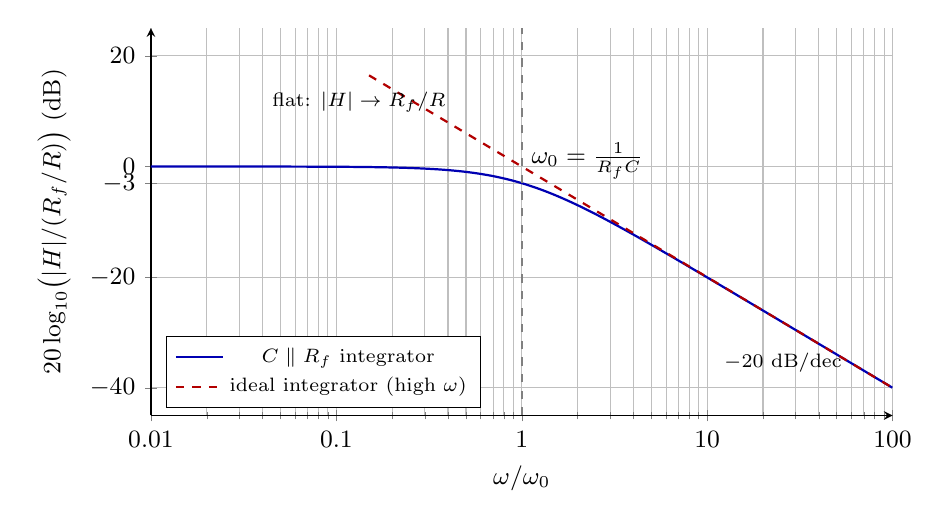
\begin{tikzpicture}
  \begin{axis}[
    width=11cm,
    height=6.5cm,
    xmode=log,
    xmin=1e-2,
    xmax=1e2,
    ymin=-45,
    ymax=25,
    axis lines=left,
    xlabel={$\omega/\omega_0$},
    ylabel={$20\log_{10}\bigl(|H|/(R_f/R)\bigr)$ (dB)},
    xtick={1e-2,1e-1,1,1e1,1e2},
    xticklabels={$0.01$,$0.1$,$1$,$10$,$100$},
    ytick={-40,-20,-3,0,20},
    grid=both,
    minor tick num=1,
    tick label style={font=\small},
    label style={font=\small},
    every axis plot/.append style={thick},
    legend style={font=\scriptsize,at={(0.02,0.02)},anchor=south west},
  ]
    \addplot[blue!70!black,domain=1e-2:1e2,samples=300]
      {-10*ln(1+x^2)/ln(10)};
    \addplot[red!70!black,dashed,domain=0.15:1e2,samples=200]
      {-20*ln(x)/ln(10)};
    \addplot[gray,dashed] coordinates {(1,-45) (1,25)};
    \node[anchor=south west,font=\small] at (axis cs:1,-4)
      {$\omega_0=\frac{1}{R_f C}$};
    \node[anchor=south west,font=\scriptsize] at (axis cs:0.04,8)
      {flat: $|H|\to R_f/R$};
    \node[anchor=north east,font=\scriptsize] at (axis cs:60,-32)
      {$-20$ dB/dec};
    \legend{$C\parallel R_f$ integrator, ideal integrator (high $\omega$)}
  \end{axis}
\end{tikzpicture}
\end{document}
